\documentclass[a4paper,english,12pt,bibliography=totoc]{scrreprt}
\setlength{\parindent}{0pt}
\usepackage[T1]{fontenc} %immer
\usepackage[utf8]{inputenc} %am
\usepackage{babel} %Anfang

\usepackage{enumitem} %Aufzählungen verändern

%Gleichungen verwenden
\usepackage{newtxtext}
\usepackage{amsmath}
\usepackage{amssymb}
\usepackage{mathptmx}
%\usepackage{txfonts}

\usepackage{listings}% code blocks
\usepackage[most]{tcolorbox}

%Querverweise
\usepackage{varioref} %immer
\usepackage{hyperref} %in dieser
\usepackage{cleveref} %Reihenfolge

\usepackage{booktabs} %schönere Tabellen
\usepackage{siunitx} %SI-Einheiten
\usepackage{tabularx} %Tabellen mit flexiblen Spalten	

\usepackage{graphicx} %Grafiken verwenden

\usepackage{lipsum} %Blindtext
\usepackage{subcaption}
\usepackage{afterpage}
\usepackage[headsepline]{scrlayer-scrpage} %Paket für Kopfzeilen
\usepackage{afterpage}
\usepackage{float}
\automark[subsection]{section}

\pagestyle{scrheadings}
\ihead{} % oben links
\chead{\leftmark} % oben Mitte
\ohead{} % oben rechts
\cfoot{\pagemark} % unten Mitte
\automark[section]{section} % Modified line

% Zu volle hboxen korrigieren
\tolerance 1414
\hbadness 1414
\emergencystretch 1.5em
\hfuzz 0.3pt
\widowpenalty=10000
\vfuzz \hfuzz
\raggedbottom

%Informationen über das Dokument
\date{\today}


\begin{document}


\begin{titlepage}
	\centering
	
\includegraphics[width=0.8\textwidth]{logo_uulm_sw}
	
	\vspace{1cm}
	\LARGE Compulsory Module for Master Programs
	\Huge \textbf{Biophysics Lab Course}
	
	\vspace{1cm}
	\Large Experiment:

	\Huge \textbf{Protein crystalization}
	
	\vspace{15mm}
	\Large Performed on 11.12.2023
	
	\vspace{5mm}
	\LARGE Group 8
	
	\vspace{1cm}
	\Large
	\begin{tabular}{rcl}
	\textbf{Haiyang Zhang} & and & \textbf{Nicolae Turcan}\\
	\href{mailto:student.1@uni-ulm.de}{haiyang.zhang@uni-ulm.de} & & \href{mailto:student.2@uni-ulm.de}{nicolae.turcan@uni-ulm.de}
	\end{tabular}
	
	\vspace{7mm}
	Supervisor: David Sinn
	
	\vfill
	\begin{tabular}{p{50mm}@{\hspace{5cm}}p{50mm}}
	\centering \underline{Haiyang Zhang} & \centering \underline{Nicolae Turcan} 
	%\hrulefill & \hrulefill 
	\end{tabular}
	
	\vspace{5mm}
	\normalsize \raggedright
	We hereby confirm that we have elaborated the present work independently and have detailed knowledge of the entire contents.
\end{titlepage}

\tableofcontents

\chapter{Introduction}

Since late 19th century, protein crystallization was already developed as a powerful purification tool and demonstration of chemical purity. Single protein crystals are necessary for X-ray and neutron diffractions, which are very essential techniques to yield atomic level structural images of biological macromolecules.\hyperref[sec:ref_1]{[1]} However, unlike the procedure of acquiring some simple inorganic crystals, protein crystallization has two challenges.\\


\begin{figure}[H]
        \centering
        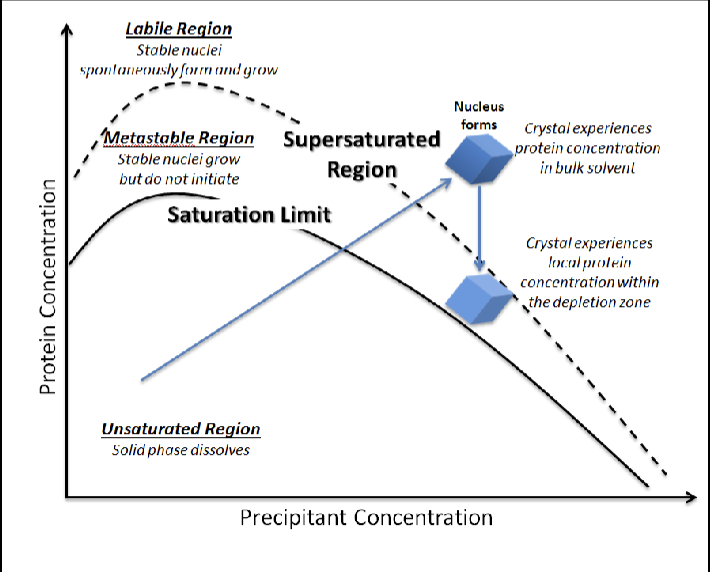
\includegraphics[width=0.9\textwidth]{2. First draft of protein crystalization/Images/Crystalization curves.png}
	    \caption{Phase diagram for the description of protein crystallization}
\end{figure}

First of all, for biological macro-molecules crystallization, very pure protein solution is a necessary prerequisite. However, the purification of protein solution is difficult. The following properties of protein, such as the complexity of the protein structure, easy to be influenced by internal and external factors and easy to be degraded makes it a difficult task to purify them without damaging the structural integrity and biological activity.  In this case, many purification strategies are made on the basis of the unique physical and chemical properties, and the 3-D structures of the target proteins.\hyperref[sec:ref_2]{[2]}.\\

Furthermore, overcome the nucleation barrier is another challenge in protein crystallization. Generally speaking, supersaturated solutions are necessary for the nucleation. However, it is more likely to form many small crystals instead of large crystals if the solution is supersaturated throughout the entire process. In order to grow large crystals, the solution should be kept in the metastable region, where no nuclei will be formed. As is shown in the figure 1.1\hyperref[sec:ref_3]{[3]}, the approach involves initiating nucleation in a supersaturated state initially. Subsequently, the solution is carefully manipulated to transition into a metastable state, fostering the growth of crystals.\\

In our experiment, we used the Vapor diffusion techniques(see methods part) to control the solution of the protein, and by attempting different combinations of NaCl solution and sodium acetatewhich, alter the solubility of the protein, we aimed to identify the optimal conditions for protein crystallization.

\chapter{Materials and methods}

\section{Materials}

\begin{table}[h]
\centering
\begin{tabular}{|c|c|}
  \hline
  Material name & model \\
  \hline
  Lysozyme in \(\mathrm{H_2O }\) & 20 mg/ml \\
    \hline
  NaCl solution & 20\%  \\
    \hline
  Distilled water &  \\
    \hline
Sodium acetate & 250mM, pH4.0\\
  \hline
  Sodium acetate & 250mM, pH4.4\\
  \hline
  Sodium acetate & 250mM, pH4.8\\
  \hline
  Sodium acetate & 250mM, pH5.2\\
  \hline
  FutureWinJoe & \\
  \hline
\end{tabular}
\caption{Materials}
\label{tab:material}
\end{table}

\begin{figure}[H]
        \centering
        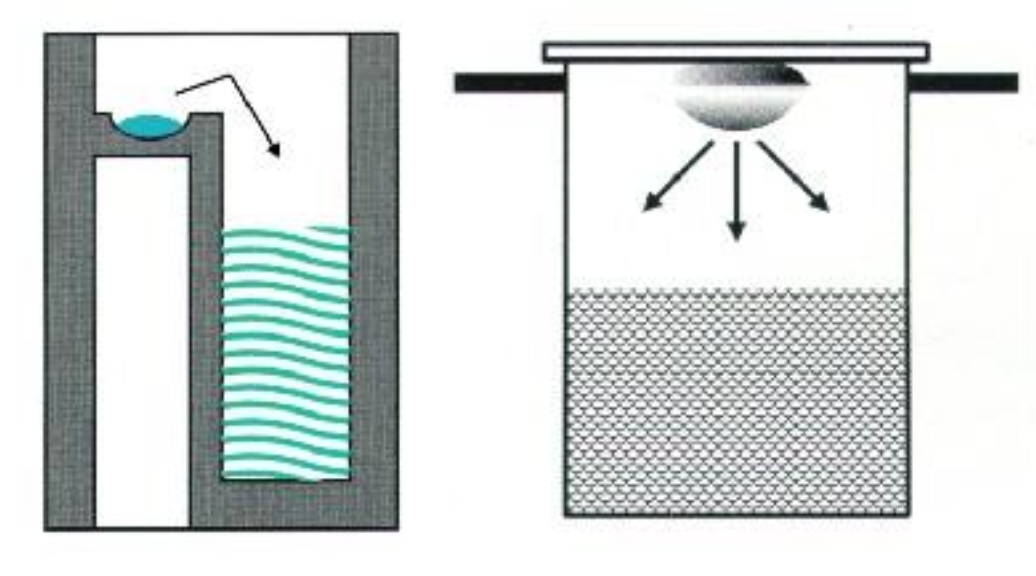
\includegraphics[width=0.8\textwidth]{2. First draft of protein crystalization/Images/Vapour diffusion techniques.png}
	    \caption{The vapor diffusion crystallization techniques: sitting drop(left) and hanging drop(right)}
\end{figure}

\begin{figure}[H]
        \centering
        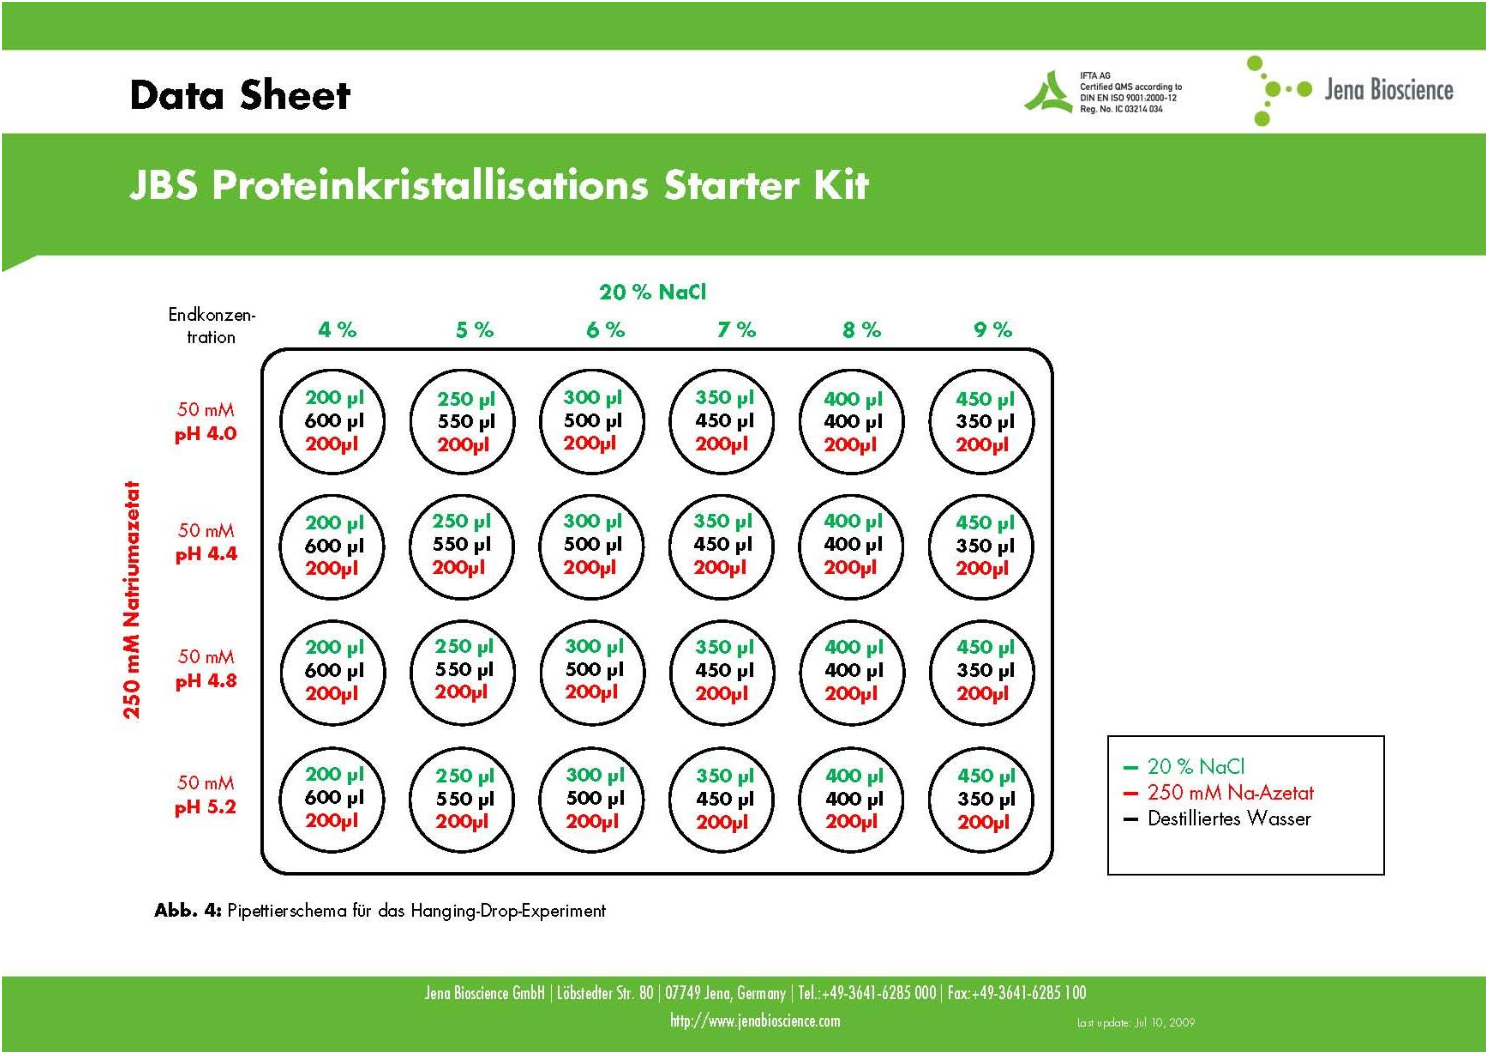
\includegraphics[width=0.8\textwidth]{wells}
	    \caption{pH and NaCl concentration of buffer in each well}
\end{figure}

\section{Methods}
Vapor diffusion technique were developed in this experiment.(Figure 2.1\hyperref[sec:ref_3]{[3]}) In this technique, a droplet mixed with purified protien, buffer and precipitant is sealed together in a chamber. The transfer of water from the droplet to reservoir will happen because of the 
droplet have a higher concentration of precipitant. As the concentration of protein in the droplet increasing, the nucleation barrier is exceeded, which is necessary for nucleation. After that, the concentration of protein solution will decrease, and ideally it will approach the metastable region, and starting to form the large crystal. In the figure 2.1, two methods(sitting drop and hanging drop) are shown in the figure, and hanging drop method is applied in our experiment.\\


In this experiment, we pipette three different solutions into the \(4 \times 6\)  well plate according to the figure 2.2, then we put a ring of silicone grease around each well. After that, 1\(\mu l\) of protein solution and 1\(\mu l\) of buffer from the respective well are mixed on the middle of the cover slip. More over, we turn over the cover slips and place them on each well. Finally, we put the plate under room temperature for protein crystallisation.


\chapter{Result and discussion}
After 48 hours, we could not find any protein crystal by direct inspection. However, we observed some differences about the size of crystals and the distribution of the protein crystals in the solution using FutureWinJoe. The situation are demonstrated in the table 3.1.

\begin{table}[h]
\centering
\begin{tabular}{|c|c|c|c|c|c|c|}
  \hline
   concentration of NaCl/ pH& \%4 & \%5 & \%6 & \%7 &\%8 & \%9 \\
    \hline
	pH 4.0 &Ms &Ms & Ms& Ms+Fl &Ms+Fl &Ss+Fl \\
  \hline
  	pH 4.4 &Ss+Fl &Ms &Ms+Fl &Ms &Ms &Ss+Fl \\
  \hline
        pH 4.8 &Ms+Fl &Ms &Ms & Ms+Fl&Ms+Fl & Ms+Fl\\
  \hline
        pH 5.2 &Fs+Fl &Fs & Ms &Ms &Ms &Fs \\
  \hline
\end{tabular}
\caption{Situations of protein crystals in each well, M means many, S means some, F means few, l means large, s means small. For example, Ms+fl means in the drop there are many small crystals and a few of large crystals in this droplet.}
\end{table}


In this context, 'many' indicates that the droplet is nearly fully occupied by crystals, while 'some crystals' suggests a more dispersed distribution. 'Few' signifies that only a small number of crystals are present within the droplet. In terms of crystal size, 'small' refers to crystals with a size smaller than 50 $\mu$m, whereas 'large' indicates crystals larger than 50$\mu$m. Examples illustrating these distinctions are presented in Figure 3.1.


\begin{figure}[H]

    \begin{subfigure}{0.45\textwidth}
        \centering
        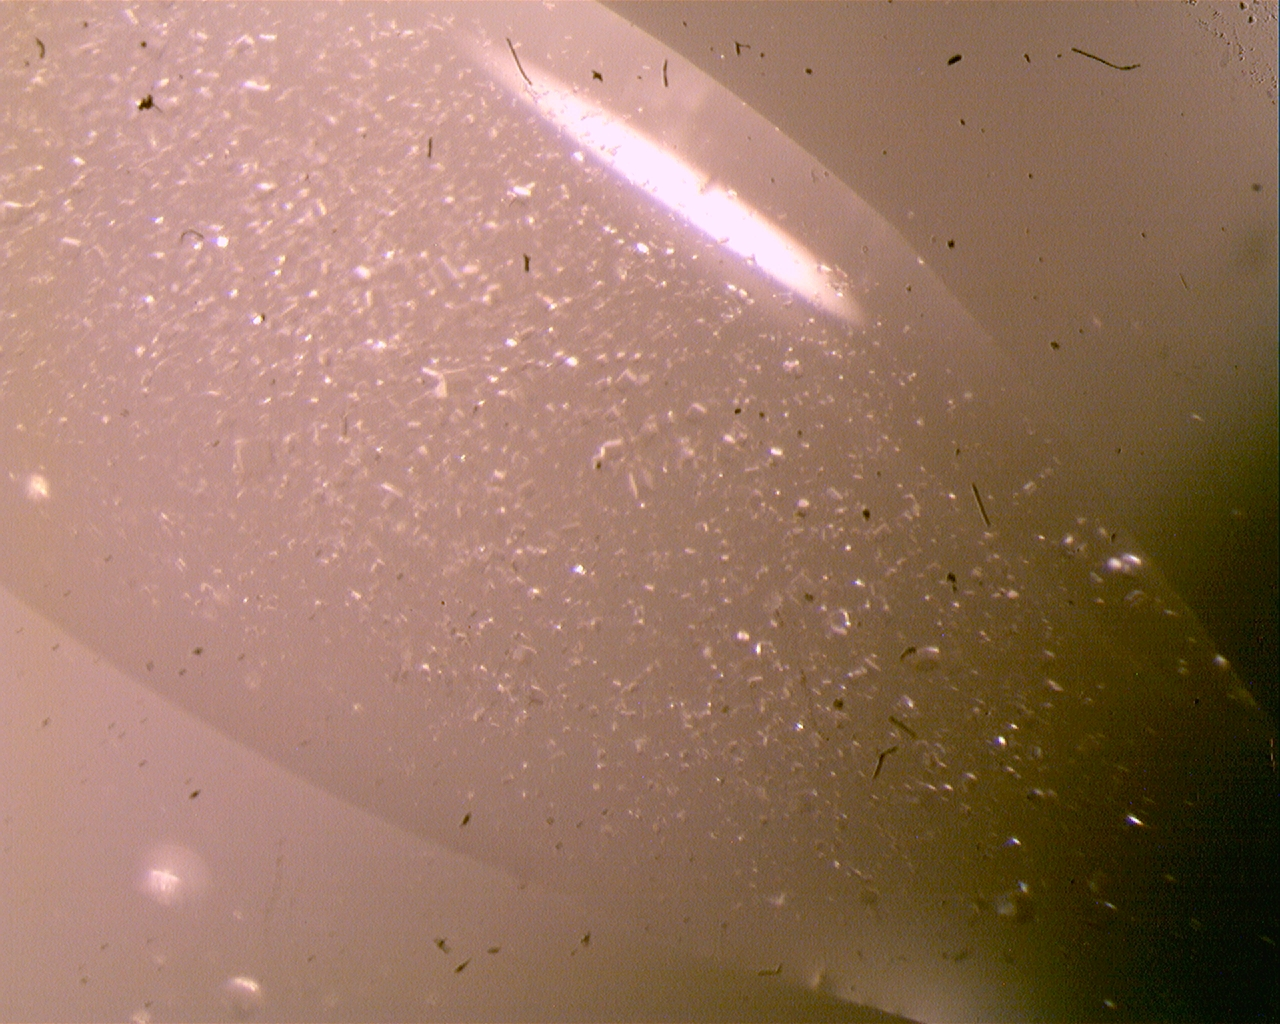
\includegraphics[width=\textwidth]{2. First draft of protein crystalization/Images/Image-6_2000-01-21.jpg}
        \caption{The crystal distribution in the droplet where pH = 4.4 and concentration of NaCl = 4\%}
        \label{fig:pH4.4,4ptg}
    \end{subfigure}
    \begin{subfigure}{0.45\textwidth}
        \centering
        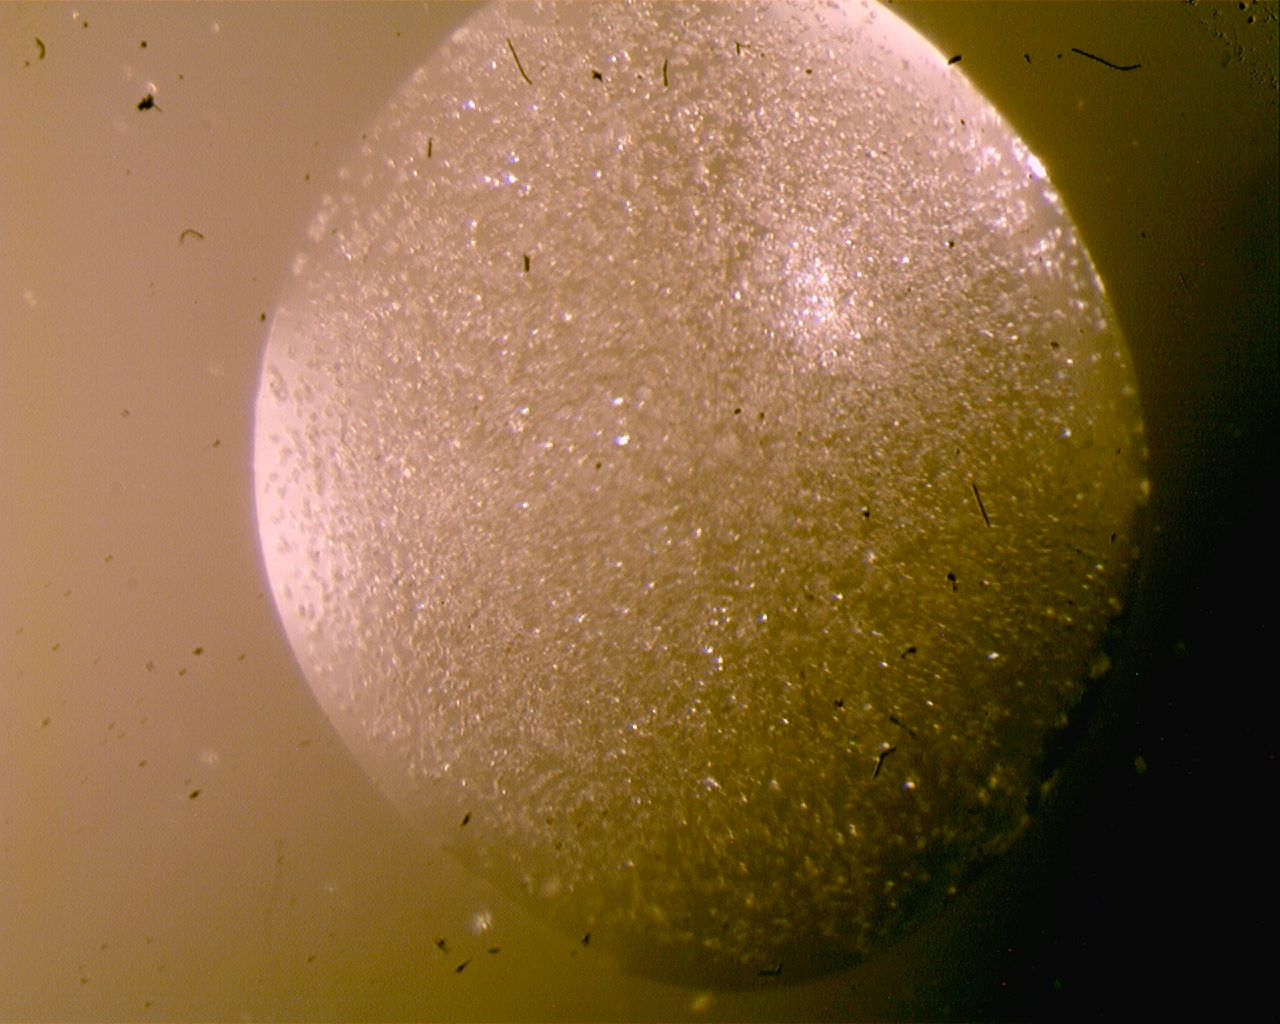
\includegraphics[width=\textwidth]{2. First draft of protein crystalization/Images/Image-9_2000-01-21.jpg}
        \caption{The crystal distribution in the droplet where pH = 4.4 and concentration of NaCl = 7\%}
        \label{fig:pH4.4,7ptg}
    \end{subfigure}
    \caption{The crystal distribution in the droplet. The left one is described as some small crystals and few large crystals; the right one is described as many small crystals. }
    \label{fig:ym_cp_curve}
    
\end{figure}

According to previous research, the pH and the concentration of NaCl solution has evident influence on the solubility of protein.\hyperref[sec:ref_4]{[4]}. Applying the mechanics of crystallization mentioned in the introduction part, we are giving a brief discussion on the results shown in table 3.1.\\

After the transfer of water molecules into the chamber, nucleation occurs in the supersaturated region. In this process, many small nuclei will appear. Subsequently, as the protein concentration decreases, the protein solution reaches the metastable region. Here, the crystals begin to grow larger, and growth halts when the concentration of the solution equals the saturation limit. The analysis of each group (separated by pH) is as follows:\\

-pH = 4.0: All protein solutions start in the supersaturated region. Between 4\% NaCl and 6\% NaCl, the solubility of the protein is relatively low as the solution remains in the supersaturated region post-nucleation. However, from the 7\% NaCl, as the concentration of the NaCl solution increases, the solubility of the protein also increases. The protein solution transitions into the metastable region, leading to the formation of large crystals.\\

\begin{figure}[H]
        \centering
        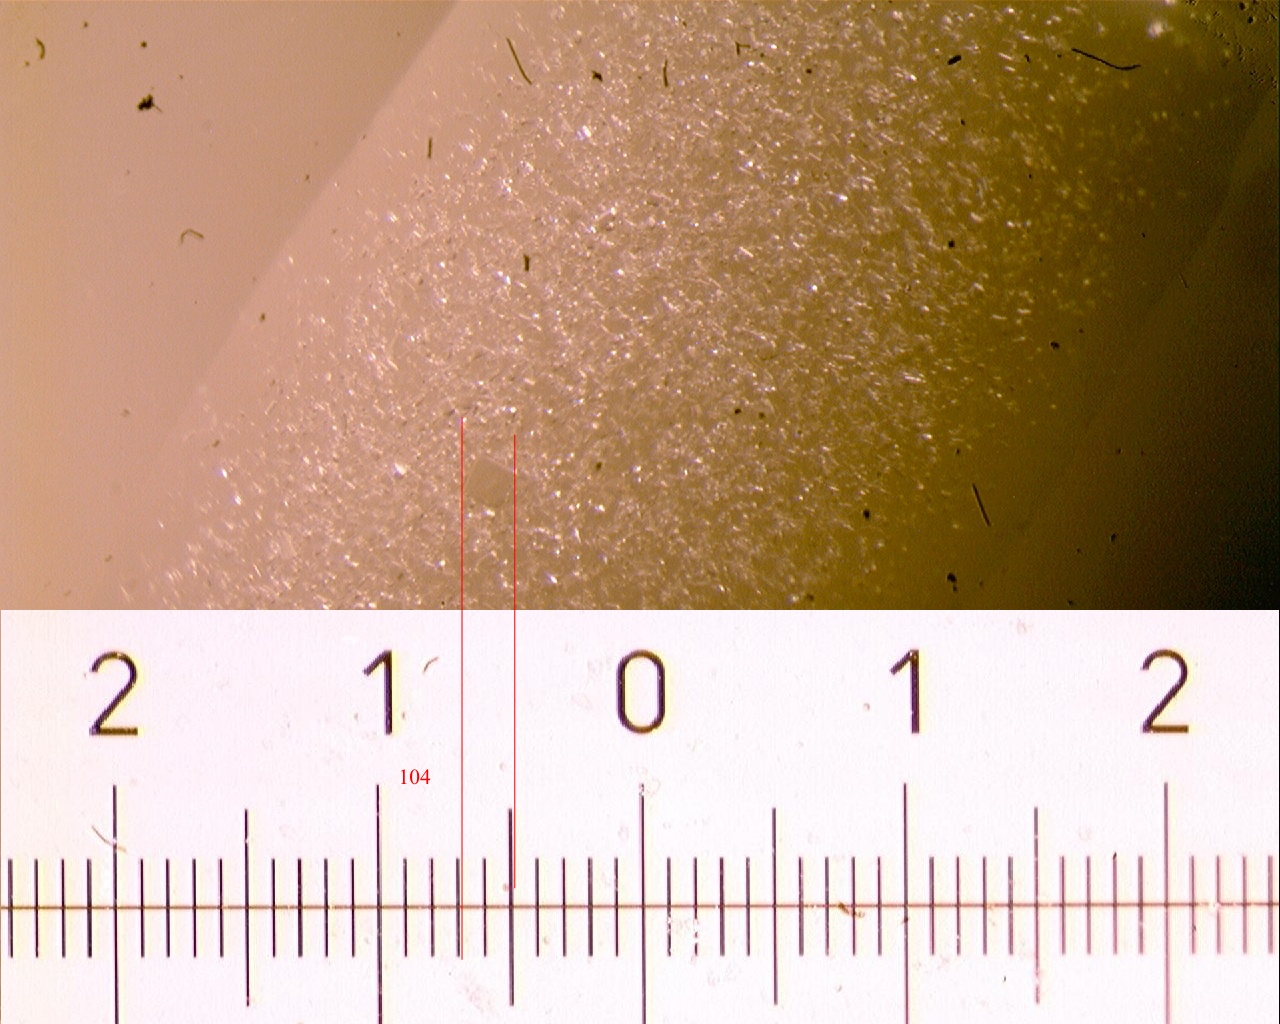
\includegraphics[width=0.9\textwidth]{2. First draft of protein crystalization/Images/labelled-Image-8_2000-01-21.jpg}
	    \caption{The largest crystal}
\end{figure}

-pH = 4.4: All protein solutions start in the supersaturated region. However, the solubility of the protein is higher under 4\% NaCl, 6\% NaCl and 9\% NaCl, indicating that the protein solution will transition into the metastable region after nucleation.\\

-pH = 4.8: All protein solutions start in the supersaturated region. However, the solubility of the protein is higher under 4\% NaCl, 7\% NaCl, 8\% NaCl and 9\% NaCl, indicating that the protein solution will transition into the metastable region after nucleation.\\


-pH = 5.2: All protein solutions start in the supersaturated region. The conditions of the solution under 4\% NaCl, 5\% NaCl and 9\% NaCl are at the edge of the supersaturated region, indicating that only a few nuclei are formed. In the other solutions, the concentration of protein remain in the supersaturated region after 24 hours.\\

Finally, the largest crystal was found at the pH = 4.4, 6\% NaCl, with the length equals to 104$\pm $2$\mu$m.(Figure 3.2)\\

According to the previous study\hyperref[sec:ref_4]{[4]}, the solubility of protein changes regular, and linear within a certain range, which is contradict to the results in our experiment. The reason of this situation may be that the well is not perfectly sealed, which will influence the transferring of water molecular; it is hard to transfer 10 $\mu$l solution using the pipettes in the lab, which may influence the ratio of protein solution and buffer. Using a better sealing skill and a better pipette will be the solution of these problems.

\chapter{Reference}
[1]\label{sec:ref_1} : McPherson A, Gavira JA. Introduction to protein crystallization. Acta Crystallogr F Struct Biol Commun. 2014 Jan;70(Pt 1):2-20. doi: 10.1107/S2053230X13033141. Epub 2013 Dec 24. PMID: 24419610; PMCID: PMC3943105. \\

[2]\label{sec:ref_2} : Du M, Hou Z, Liu L, Xuan Y, Chen X, Fan L, Li Z, Xu B. 1Progress, applications, challenges and prospects of protein purification technology. Front Bioeng Biotechnol. 2022 Dec 6;10:1028691. doi: 10.3389/fbioe.2022.1028691. PMID: 36561042; PMCID: PMC9763899.\\

[3]\label{sec:ref_3} : Protein Crystallization, Biophysics lab course, Ulm University.\\

[4]\label{sec:ref_4} : Aduja Naik, G.V. Venu, Maya Prakash \& K.S.M.S. Raghavarao. (2014) Dehydration of coconut skim milk and evaluation of functional properties. CyTA - Journal of Food 12:3, pages 227-234.\\

%[5]\label{sec:ref_5} : 
\end{document}
